\documentclass[crop,tikz]{standalone}
\usetikzlibrary{backgrounds}
\colorlet{blue}{cyan}
\tikzset{ inverted/.style={every path/.style={draw=white,text=white}, background rectangle/.style={fill}, show background rectangle }}

\tikzset{>=latex}
\usetikzlibrary{decorations.markings}
\colorlet{green}{green}
\definecolor{orange}{RGB}{250,194,25}
\newcommand{\place}{\vec{r}}
\newcommand{\velocity}{\vec{v}}
\newcommand{\acceleration}{\vec{a}}

\begin{document}
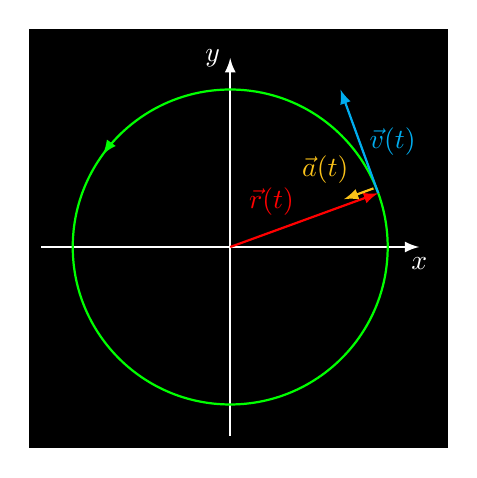
\begin{tikzpicture}[inverted,scale=2]
  % axes
  \draw[->,thick] (-1.2,0) -- (1.2,0) node[below] {$x$};
  \draw[->,thick] (0,-1.2) -- (0,1.2) node[left] {$y$};
  % circle
  \draw[
    decoration={markings, mark=at position 0.4 with {\arrow{>}}},
    postaction={decorate},
    green,
    thick
  ] (0,0) circle (1);
  % place, velocity, acceleration
  \draw[->,thick,red] (0,0) -- node[left,anchor=south east,yshift=-0.2em]{$\place(t)$} (20:1);
  \draw[->,thick,blue] (20:1) -- node[right,anchor=west]{$\velocity(t)$} +(20+90:0.7);
  \begin{scope}[shift={(-0.03,0.03)}]
    \draw[->,thick,orange] (20:1) -- node[left, anchor=south east] {$\acceleration(t)$} (20:0.8);
  \end{scope}
\end{tikzpicture}
\end{document}
